\section{Architecture}
\label{sec:architecture}

\subsection{SNC}
The SNC module is a constitutive element underlying the PE design. Since the NOC network is not
designed to ensure the maintenance of correct packet ordering, an imperative design consideration is to
evade out-of-order packet delivery by storing and reassembling the incoming packets. Upon sending
input layer data, sending environment assigns each packet a sequence number which is entered into the
seqNum field. However, it is worth to note that the number being assigned corresponds to the session
number rather than to a single packet i.e a vector comprising n input layer data will be sent in n packets
with same sequence number. After processing the input data, the output packet from PE retains
sequence number of the input packets. The individual units of input layer data are differentiated using
index field, while individual hidden and output layer packets are differentiated using sourceAddress
field.

\begin{figure}
    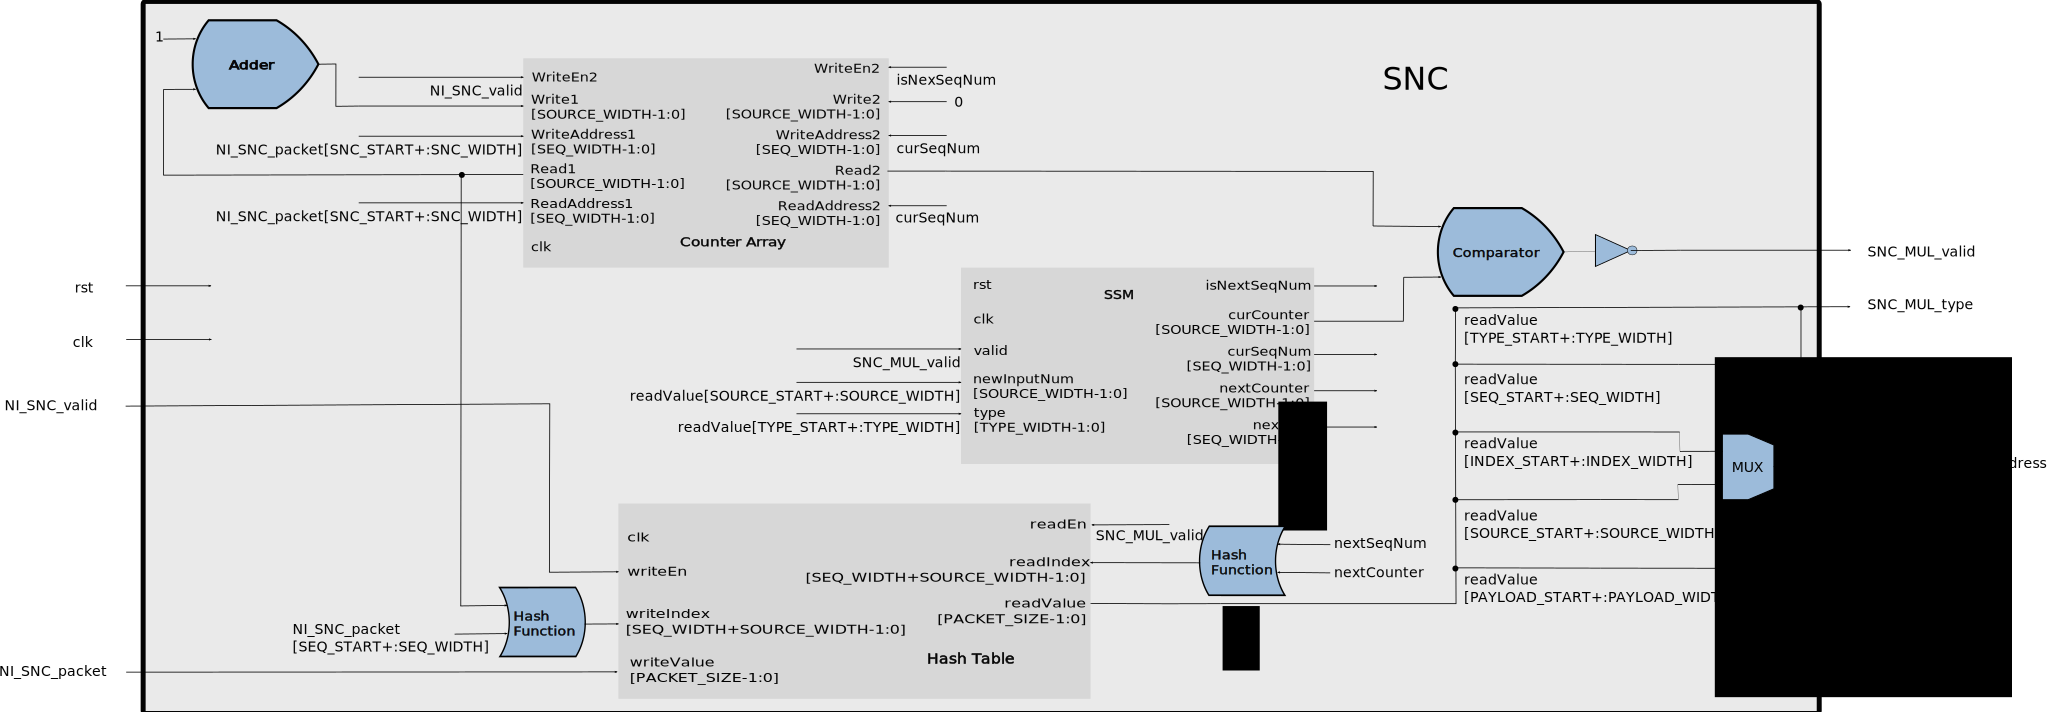
\includegraphics[width=\textwidth]{Figures/snc.pdf}
    \caption{SNC Architecture} 
    \label{figure:snc}
\end{figure}

The figure~\ref{figure:snc} depicts SNC hardware block diagram. The packets arriving from the network
interface are first stored in the hash table (HT) memory. The memory consists of $2^{SEQ_WIDTH}$ blocks,
where $SEQ_WIDTH$ amounts to the number of bits in the packet’s seqNum field. For the sake of full
configurability, for the given NOC of size $NETWORK_SIZE$, each PE can be configured to receive inputs
from up to $NETWORK_SIZE$ terminals. Thus, every block is further divided to contain place for
$NETWORK_SIZE$ packets. The packets are mapped into memory through hash function, where
hf (seqNum, counter[seqNum]) = concatenate (seqNum, counter[seqNum]);
Here, the counter[seqNum] embodies the number of packets with the given sequence number that have
arrived to PE and is stored in counter array (CR). After the packet is mapped into appropriate position
within HT, the counter [seqNum] is incremented, so that the next packets with the same sequence
number is stored in the next memory location. The SNC State Machine (SSM) (Figure /ref{figure:sst})
tracks current sequence number and counter to retrieve packets from the HT. The number of inputs
linked to PE is configured using corresponding control packet.

\begin{figure}
    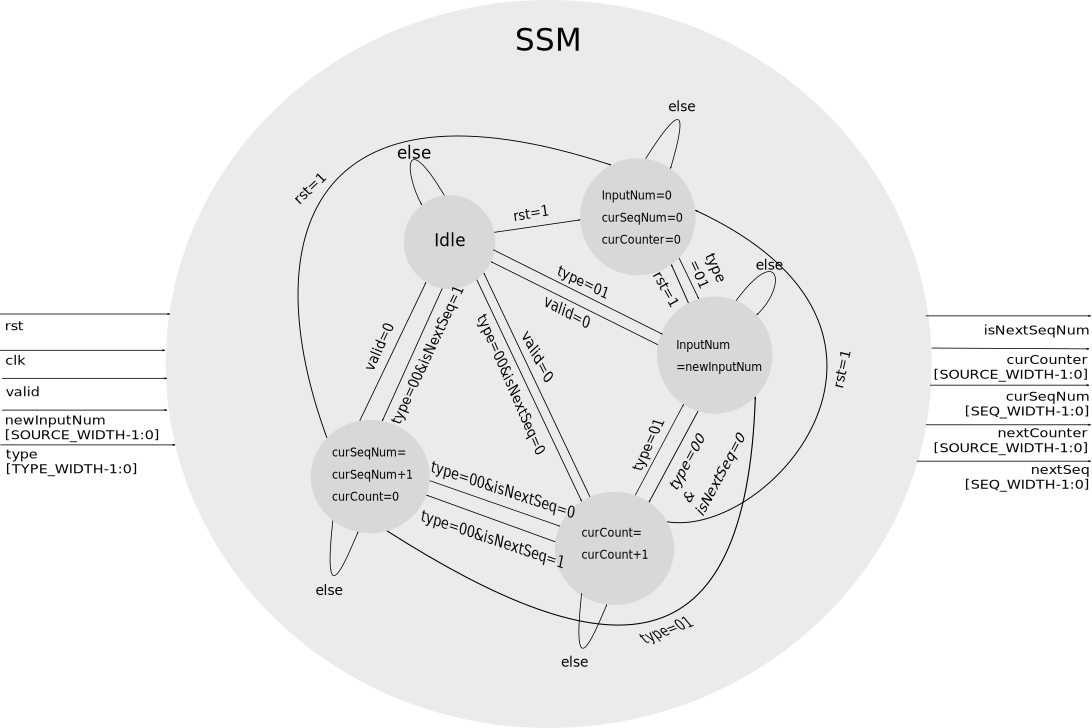
\includegraphics[width=\textwidth]{Figures/sst.pdf}
    \caption{SST} 
    \label{figure:sst}
\end{figure}
